\documentclass[10pt,a4paper,twoside]{article}

\usepackage{vmargin,fancyheadings,multicol,multirow,ifthen,cite,
            graphicx,wrapfig,calc,dcolumn,apalike,setspace,
            boxedminipage,rotating,textcomp,picinpar,longtable,
            url,amsmath,amssymb,ogonek} 

\usepackage[tight]{subfigure}
\usepackage{imc2018}

\begin{document}
\SetPaperBodyFont

\begin{IMCpaper}{
\title{Title of this paper}
\author{Silvia~Sheep$^1$, T.~Eddy Bear$^1$, Benny I.~G. Bear$^2$, and
  Catharina C\"ow$^3$
        \thanks{$^1\,$Green Meadow Observatory, Prairieland Street,
          Littletown, LT61 1AB, 
                Northern Ireland\\
                     \texttt{ssheep@arm.ac.uk} \mbox{\rm and}
                     \texttt{tbear@arm.ac.uk}\\[1ex]
                $^2\,$Research Institute of Applied Mathematics and
                      Mechanics of Tomsk State University,\\
                      Tomsk, Russia\\ 
                     \texttt{big.bear@tomskuniversity.ru}\\[1ex]
                $^3\,$Leiden Observatory, Leiden University,
                     Kalverstraat 27, 3502 XY Leiden\\
                     \texttt{cc@leidenuniversity.nl}}}%
\abstract{This is a template for a paper or a poster to be presented at the
  International Meteor Conference in Pezinok-Modra, Slovakia, from
  August~30 to September~1, 2018. Besides being a template, this
  document also contains information for the preparation of your
  paper, complementing the \emph{Instructions for all authors\/} on the IMC
  2018 web pages.}}%  
\index{Sheep S.}%
\index{Bear T.~E.}%
\index{Bear B.~I.G.}%
\index{Cow@C\"ow C.}%
\vspace*{-3\baselineskip}
\section{Introduction}
This article presents how to make a correct paper with pictures and
tables. At the end are also examples of references. First of all,
notice the file name. We use a uniform naming scheme consisting of the
year (in this case, \texttt{2018}), the number assigned to your paper
(in this case \texttt{L12}), and the last name of the corresponding
author in all-lowercase characters (in this case \texttt{sheep}), all
separated by hyphens. Please adhere to this format; that makes life simpler
to us!

The editors will edit each paper received for content, language,
style, and overall uniformity of the entire proceedings volume. The
better you prepare your man\-u\-script and the more you adhere to the
guidelines, the fewer work this will be, and the editors will be
grateful to you for that. Nevertheless, do not be overly perfectionist
either. Small changes in the final editing may have significant
implications on the layout, and it would be a pity that painstaking
finetuning efforts would prove futile in the end.

We have no formal page limits for an article, but know that most
authors manage with four pages or less. If you need more than six
pages, however, and you can justify why you need so many pages, please
contact the editors to find out whether there is room to accommodate a
paper of that length.

\section{How to make a picture}
Here is a an example of a picture
(Figure~\ref{2018-L12-sheep-figure1}). \LaTeX\ users should always use
cross-references to refer to to figures. We have a uniform scheme for
labeling figures, reminiscent of the scheme for naming files.  Please
adhere to this scheme, also for the name of the figure file!
\textsc{Pdf}\LaTeX\ accepts \texttt{.png}, \texttt{.jpg}, and
\texttt{.pdf}. We give an example of each of them in this template
article. However, always provide us with the original version of your
figure as well if it has another format. Sometimes, this helps us to
generate a better-quality conversion, if needed.  Nevertheless, the
responsibility for the quality of the picture is first and foremost
the authors': the editors can only improve what is already in the
picture in the first place! In particular, mind that it is very annyoing
for the reader to see text in a figure that is not or only poorly
readable! Also mind that the printed version of the proceedings is
produced in black and white: colors in a graph may look nice in the
on-line version, but make sure that you design your graph in such a
way that no information is lost in the printed black-and-white
version.

\begin{figure}[htb]
\centering

\includegraphics[width = \columnwidth]{2018-L12-sheep-figure1}%
\vspace*{3pt}%
\caption{The logo of the IMC 2018 is in PNG format. There is no need
  to mention the extension in the \texttt{$\backslash$includegraphics}
  command.}
\label{2018-L12-sheep-figure1}
\end{figure}

As a general rule, we print figures column-wide, as
Figure~\ref{2018-L12-sheep-figure1}. In some cases, however, this may
lead to such as small scale that essential details are lost. In this
case, you may instead create a figure that spans both columns. Notice
that the ``\texttt{h}'' and ``\texttt{b}'' options are not available
to position these large figures. Finally, if a figure is composed of
several subfigures, the \texttt{subfigure} package may be used to
arrange them properly. Figure~\ref{2018-L12-sheep-figure2} is an
example of such a figure.

\begin{figure*}[!t]
\centering
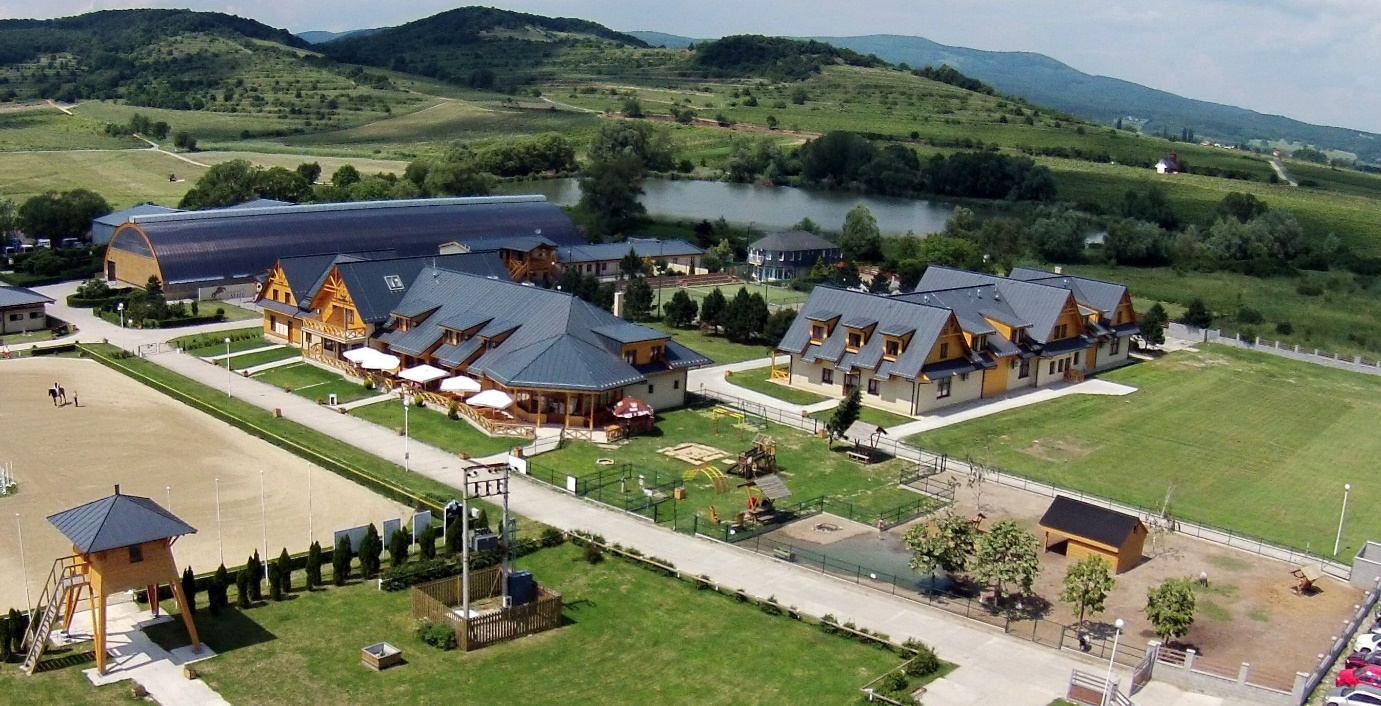
\includegraphics[width = \textwidth]{2018-L12-sheep-figure2}%
\vspace*{3pt}%
\caption{This JPEG picture of Hotel Rozalka and its vicinity contain so
  many details that we have chosen to make it span both columns. This
  option should be used sparingly, however!}
\label{2018-L12-sheep-figure2}
\end{figure*}

\section{How to write a table}
Table~\ref{2018-L12-sheep-table1} shows an example of a
\LaTeX\ table. As for figures, always use crossreferences to refer to
tables. The format of the label, \texttt{2018-L12-sheep-figure2} in
this example, is very similar to that of figures.

\begin{table}[!h]
\caption{Numbers of different kinds of participants expected to attend
  the IMC 2018.}%
\label{2018-L12-sheep-table1}
\vspace*{6pt}
\centering
\def\0{\ensuremath{\phantom{0}}}%
\def\1{\ensuremath{\phantom{.0}}}%
\begin{tabular}{lc}
\hline 
Species&Number\\
\hline
Sheep       &\0\03\\
Teddy bears & \087\\
Big bears   &\0\07\\
Cows        & \013\\
\hline
Total       &  110\\
\hline
\end{tabular}
\end{table}

In tables, captions are placed \emph{above\/} the actual table. Also
notice the use of ``\texttt{$\backslash$0}'' to line up the
numbers. Only if a tables contains few columns, it will fit in a
column. Therefore, authors may also use the
%
\begin{verbatim}
\begin{table*}[!t]
...
\end{table*}
\end{verbatim}
%
environment to create tables that span both columns.  Notice that
vertical lines are \emph{never\/} used to separate columns!

\section{Formatting and citing references}
If you know $\mathrm{B{\scriptstyle{IB}}\!T\!_{\displaystyle E}\!X}$,
please use it. We have provided the bibliography style file
\texttt{imo2.bst} for that purpose.

The file \texttt{sheep.bib} provides examples of
references that are books (Rendtel and Arlt, 2011), journals (Asher,
2010), or proceedings papers (Egorova, 2012).\footnote{The
  \textit{Instructions for all authors\/} explain how to cite references.}
Authors are requested to replace
%
\begin{verbatim}
\bibliographystyle{imo2}
\bibliography{sheep}
\end{verbatim}
%
by the content of the file \texttt{sheep.bbl} just before submitting
the article to reduce the number of files involved.

Authors not familiar with
$\mathrm{B{\scriptstyle{IB}}\!T\!_{\displaystyle E}\!X}$ but
knowledgeable with \LaTeX\ bibliographies may write the bibliography
``from scratch'' using the relevant comments in the \emph{Instructions
  for all authors\/} as guidelines. The content of the file
\texttt{2018-L12-sheep.bbl} shows how a \LaTeX\ bibliography looks
like.

Athough we do not explicitly disallow web pages in the list of
references (e.g., Vaubaillon, 2005), we ask to avoid this, as such
references by their proper nature are unstable in the long
run. Instead, use footnotes to refer to web pages.\footnote{See also
  \url{http://imc2018.imo.net/guideline}.}

\section{Conclusions and additional remarks}
The file \texttt{2018-L12-sheep.tex} is just for those who will use
\textsc{Pdf}\LaTeX\ to write a paper for the IMC 2018 Proceedings.  If
you do not use (\textsc{Pdf})\LaTeX, do not worry, the editors will
format your paper.  However, you can still look at
\texttt{2018-L12-sheep.pdf} for an example of what a paper will look
like.

If you compile your article with the files provided here, you may
notice that the columns on the last page are not balanced, unlike in
the IMC Proceedings. Do not worry, the editors will take care of
that.\footnote{Packages such as \texttt{balance} have undesired
  side-effects and are therefore not used.}  It may also be worthwhile
considering to add the option \texttt{draft} in the first line of your
document during its preparation. You will save time, because pictures
are not imported.\footnote{Only their bounding boxes are taking into
  consideration, so that the layout is exactly the same as with the
  pictures.} In addition, lines sticking out of the margin will be
marked by black boxes.

\section*{Acknowledgements and diclaimer}
The editors wish to thank David J.~Asher. His template and
instructions for the 2010 Proceedings were the basis of this adapted
version. In his honor, we include (a slight variation of) the picture
that adorned previous versions of this template.

Thanks also to all authors who will use this template to ease the
editors' work.

\begin{figure}[!t]
  \centering
\includegraphics[width = \columnwidth]{2018-L12-sheep-figure3}%
\vspace*{3pt}
\caption{This very cute creature has illustrated \LaTeX\ instructions
  for contributions to the IMC Proceedings ever since the 2010 edition in
  Armagh, as it is so endeering to both authors and
  editors. Therefore, it has become an IMC classic. This time, the
  figure is in PDF format.}%
\label{2018-L12-sheep-figure3}
\end{figure}

Finally, every resemblance between names, places, and situations
referred to in this paper and actual names, places, and situations is
unintentional and should be regarded as purely coincidental.

\nocite{*}
\bibliographystyle{imo2}
\bibliography{sheep}

\end{IMCpaper}
\end{document}
